\section{Actividad 3}

\subsection*{Se tiene la función de densidad de la Fig. \ref{fig:diagrama_3}}

    \begin{figure}[H]
        \centering
        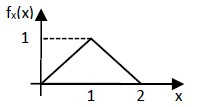
\includegraphics[width=0.3\linewidth]{imagenes/Actividad_3/actividad_3.jpg}
        \caption{Función de densidad.}
        \label{fig:diagrama_3}
    \end{figure}

\subsection*{a) Calcular analíticamente la media, la varianza y la desviación estándar.}


\subsection*{b) Calcular y graficar la función de distribución acumulada.}


\subsection*{c) Calcular \( P(0.75 \leq X \leq 1.75) \).}


\subsection*{d) Realizar un código que permita generar vector de 500 muestras aleatorias y graficar el histograma de esas muestras. Luego calcular la media 
y la varianza.}
